Our IPC implementation from Milestone 4 only handles processes that are running on the same core. With the introduction of multicore support in Milestone 5, we now must handle the case where processes are talking to each other \textit{across cores}. Remember that Barrelfish is built as a distributed operating system; this issue is paramount to reaching a fully-fledged system and we tackle it in this Milestone.

\subsection{Design Constraints}
In Milestone 4 we used LMP. Our goal now is to use ``User-Level Message Passing" (UMP) to achieve cross-core communication. UMP uses shared memory (URPC frames, one per connection) to pass messages, and supports full-duplex communication through 2 unidirectional channels (one for sending and one for receiving). For performance purposes, it avoids kernel context switches (hence ``user-level"), and communicates purely through cache lines when possible. This is possible under the assumption that our processor employs the ``MOESI" cache-coherence protocol, where reading dirty cache-lines can bypass a write-back to memory by obtaining the cache line directly from the core that ``owns" the cache-line \cite{armman}.
\\\\
Since we already implemented a messaging layer previously, our main goal in this Milestone was to implement UMP. Our design choices here mainly lent themselves to speed because IPC is crucial to many multikernel operations, and we wanted to use UMP over LMP whenever possible. As always there was a time constraint, so we also opted for simple design choices in place of more complex ones. Finally, we needed to keep in mind that both UMP and LMP are transparent to userspace processes, so it is our decision on which protocol various processes will use to communicate. Going in, the main challenges we identified were:
\begin{itemize}[itemsep=0pt]
    \item How does one bind to a service running on another core?
    \item How should the URPC frame be arranged for message passing? Where does a message start, and how long will it be?
    \item If a message is ready to be sent/received, how does the other side know? We need to guarantee that what we're reading is actually a new message, otherwise we might end up re-reading old ones. Likewise, we might end up overwriting unread messages on the sending side.
    \item Messages could possibly be larger than what UMP supports in a single send, or larger than the entire URPC frame itself. What do we do in this case? This was done in Milestone 4 with our messaging layer, but we realized that our implementation was not ambivalent to the underlying transport layer (more on this later).
    \item We currently have one instance of each resource server running (e.g. each core has its own process manager, memory manager, and serial server). How should we coordinate and synchronize them?
\end{itemize}

\subsection{Binding}
Assume that a process \textbf{A} on core \textbf{1} wants to talk to a service \textbf{B} on core \textbf{0}. Recall that in Milestone 5, \texttt{init} on core 1 is given the physical address of a frame by \texttt{init} on core 0 to set up as the URPC frame, allowing them to communicate. This only works because \texttt{init} is a privileged process that can generate new capabilities from a given physical address (``forging"). This is where the concept of the \textit{monitor} comes in. Up until this point, we have been referring to \texttt{init} as ``just another process", with its only defining part being that it is the first process to run. In this Milestone and onwards however, we will refer to it as the ``monitor" and give it its first special job: to help processes bind to each other across cores. It is able to perform this job because of its ability to forge capabilities.
\\\\
For simplicity we have been housing all resource servers within the monitor up to this point, with the plan to separate them later in Milestone 7 when the nameserver is built. Thus, when we refer to a resource server in this section, we really mean the monitor. Suppose there is a child process, \textbf{A}, on core \textbf{1}, that wishes to communicate with a resource server on core \textbf{0}. The procedure for enabling communication between child processes and a resource server is as follows (Figure \ref{figure:m6-bind}):
\begin{enumerate}[itemsep=0pt]
    \item The child process \textbf{A} sends a frame capability (the frame in which UMP communication will occur) over LMP to its monitor (on core \textbf{1}).
    \item Core \textbf{1}'s monitor sends the \textit{physical address} of the frame to core \textbf{0}'s monitor via their UMP channel. The physical address is necessary because UMP currently cannot safely send capabilities (this changes in Milestone 7).
    \item Core \textbf{0}'s monitor forges a capability to the client frame and initializes an RPC channel to process \textbf{A}. 
    \item The client frame is split in half. From the server's point of view, one side is for sending messages, and the other is for receiving them. To the client, this view is flipped; the server's sending side is the client's receiving side, and the server's receiving side is the client's sending side. This is explained further in the following section.
\end{enumerate} 
Note that this binding procedure generalizes; one way to achieve communication between two processes across cores would be to have their respective monitors act as middle-men.
\begin{figure}[ht]
    \centering
    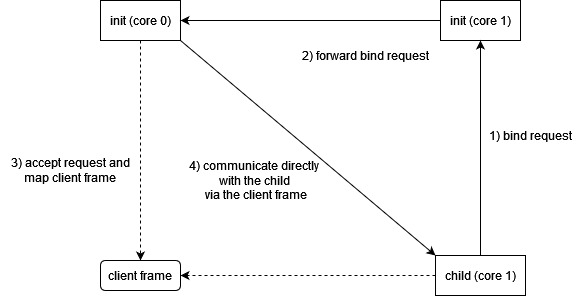
\includegraphics[width=0.8\columnwidth]{images/m6-bind.jpg}
    \caption{The sequence of events that occur during a binding request}
    \label{figure:m6-bind}
\end{figure}

\subsection{Transporting Message}
In Milestone 4 we built a generic transport interface to abstract RPC logic out from a specific transport protocol (Figure \ref{figure:m6-rpc-layout}). So, to add UMP support, we simply had to implement the generic functions for this interface without altering the RPC library functions.
\begin{figure}[ht]
    \centering
    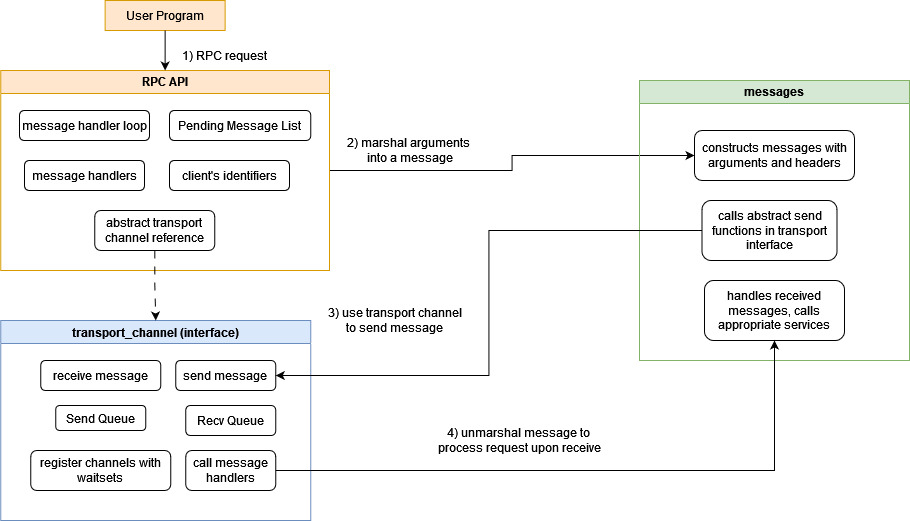
\includegraphics[width=\columnwidth]{images/m6-rpc-layout.jpg}
    \caption{The various layers involved in servicing an RPC.}
    \label{figure:m6-rpc-layout}
\end{figure}

\subsubsection{Ring Buffers}
We use a \textit{ring buffer} for UMP connections, which can be thought of as a queue that wraps back around to its start when its maximum size is reached. More specifically, we use two shared ring buffers: one for sending, and one for receiving. Since the buffers are shared between both sides of the connection, the sending buffer for one side will be the receiving buffer for the other and vice versa. Before getting any deeper, there is a bit of jargon to understand here:
\begin{itemize}[itemsep=0pt]
    \item \textbf{Slot}: A placeholder for a message in a ring buffer. This may contain the message, as well as other metadata necessary for proper handling of the message. From the perspective of the reader/writer this is atomic, just as a slot in an array is.
    \item \textbf{Waitset}: Acts as the connective tissue between threads and channels. For example, if we want to know when something is ready to be received on the channel, we use a waitset to poll for a \texttt{UMP\_IN} event, which tells us that something has been put into the receive buffer.
    \item \textbf{Control Word}: A reserved byte which each slot in a ring buffer contains. A \texttt{UMP\_IN} event only tells us that something has been written, but not if the message being written is finished, so we use the control word to do so. The control word is crucial in the synchronization of message content between the two cores, which is detailed in a later section.
\end{itemize}
On the receiving side, we use a \textit{waitset} to poll a \textit{control word} in the next \textit{receive slot}. That is, we hold a pointer into the next slot a message will be written into. Every time something is written, we check if the associated control word is set. If it is, we know that the message is ready and that we can begin to read and process it. On the sending side, we have to check if the buffer is full. If it isn't we can simply write the message (and set the control word when we're done), but if it is we use a waitset to poll until the receiver acknowledges a message.

\subsubsection{Memory Barriers}
Our system assumes an ARM processor, so we must take into account its ``weak memory consistency model``. The chip does not guarantee that memory stores/loads will occur in the order they are written by the program. This is particularly important for UMP since we use a control word between UMP clients and servers to signal whether messages are ready to be received. There is no guarantee that the sending core actually sets the control word \textit{after} it writes the message data, and similarly there is no guarantee that the client correctly checks the control word \textit{before} reading the message data. To solve this we employ the use of memory barriers, which ensure that load and stores occur in their intended order, while polling the UMP channel and receiving messages.

\subsubsection{ACKs}
How does the receiver acknowledge a message? In other words, how do we know what the receiver has and hasn't read from the ring buffer? This is necessary else we may end up overwriting unread messages, or re-reading messages that have already been read. The first idea we had was to have the receiver send an ACK over its sending buffer, signalling that a slot has been read in its receiving buffer, thus allowing the sender to reuse that slot. However, an ACK is also like any other UMP message---how do we know that an ACK has indeed been received? We can't send an ACK for a received ACK, as this clearly ends with an infinite loop. 
\\\\
One might reason that we can simply assume the ACK has been received (thus freeing that slot to be reused), however this is an unsafe assumption to make. In the case where the sender has not actually gotten around to processing the ACK and the receiver sends a bunch more messages to the point where the buffer does a full loop back around to the ACK, it will be overwritten and lost before being read.
\\\\
We figured that this problem may be solvable with extra checks and metadata, but we ended up opting for a more efficient (and arguably simpler) approach. Now, we reserve a slot in the ring buffer for ACKs (the ``ACK slot"), storing the index of the next unread slot. When the receiver reads a message from its receiving buffer, it increments the ACK slot index which points at the next unread slot. Before the sender puts a message in this buffer, it reads the ACK slot to check that the slot it is writing into doesn't contain an unread message. In order to handle cases where ACKs in the buffer have looped back around and thus overlap with the index, we use an additional piece of information in the ACK slot called the ``iteration number". This solution is a bit nicer than the previous because we always use at most 1 extra slot, no matter how many messages are sent. With the previous implementation, we required 2 slots for every 1 message sent (1 for the message, 1 more for the ACK).

\subsubsection{Large Messages}
In Milestone 4, when a message was larger than what a single send could handle, we would fill a frame with the excess data (arguments/return values) and then pass the frame's capability to the receiver. This turned out to be a major oversight on our part because UMP cannot arbitrarily pass frame capabilities in a safe manner (although Milestone 7 improves this). To do so with the current state of our system would require un-tracked forgings of capabilities on the fly, which can cause memory-consistency issues.
\\\\
In order to handle large messages (in a way that is ambivalent to the transport layer), we now have the sender split the data and send it as a series of smaller messages that each fit in a slot. The receiver accumulates the data in a buffer and forwards it to the appropriate message handler once the full message is received. Note that the message data chunks do not specify ordering because it is not necessary; this is the case because each RPC channel has its own individual waitset, which we explain next.

\subsubsection{Waitsets}
We previously used a single waitset for all RPC channels (specifically, the default waitset configured for a domain). This worked fine in Milestone 4, but it introduced a glaring problem with our system that surfaced with the introduction of UMP.
\\\\
With a singular waitset, all associated threads waiting on it will be woken up when \textit{any} channel picks up an event. If we have multiple RPC calls in flight on both LMP and UMP channels, threads that are meant to only service UMP requests will become triggered by an LMP request sent on the same waitset. This is particularly bad when we require sequences of an LMP call followed by a UMP call to service a request (e.g. during client-server binding), as the UMP handling thread will become blocked by accidentally trying to service the LMP request. Even if we somehow prevent this LMP-UMP problem, the wrong thread may continually pick up an event and then put it back on the waitset, resulting in randomly long processing times for RPCs.
\\\\
With our new message splitting scheme this becomes worse. Since multiple message handling threads might get events for the same channel, ordering and synchronization of large messages becomes an issue in the case that different threads pick up different parts of a large message. The obvious fix for us here was to refactor such that we register one waitset per RPC channel. This means that now, each thread waits on its own isolated waitset. Thus, large messages between two processes can only ever be handled by the thread it is intended for, ensuring that it will be received in order.

\subsection{Servers}
Previously, we had a single instance of each service running because we only had a single core to run them on. With the introduction of multiple cores, information required by a service may exist outside of its scope and so we must make some changes to the existing infrastructure. There are now three questions we must address with regards to our servers:
\begin{enumerate}
    \item Where will this server run? In its own process or within the monitor?
    \item Will we host this server on a single core, or will it be duplicated across cores?
    \item How will arbitrary processes communicate with this server; with LMP, or with UMP?
\end{enumerate}

\subsubsection{Memory Management}
Our memory management server starts off as distributed, but eventually devolves into a singular server. When core \textbf{1} boots up, it's given a portion of core \textbf{0}'s starting RAM capabilities. In the early stage of the system, core \textbf{1} may use this portion of RAM to service any requests, and thus the memory servers are distributed in that processes on either core will only request RAM from the memory manager on its local core. However, when core \textbf{1} inevitably runs out of this early memory, it will then begin to service any RAM requests by forwarding it via UMP to core \textbf{0}, thus the memory server becomes a single entity.
\\\\
We have also left the memory management server insidethe monitor since it is convenient for cross-core RAM requests. Core \textbf{1} must forge a capability upon receiving RAM from core \textbf{0}, and this can only be done within a privileged process, such as the monitor. As such, processes can only communicate with the memory server through LMP, as it requires involvement of their core's monitor. 
\\\\
We decided to only allow core \textbf{1} to request memory from core \textbf{0}. So, if a process on core \textbf{1} frees memory that it has used, core \textbf{0} cannot request that RAM back from core \textbf{1}. This is addressed later in Milestone 7.

\subsubsection{Serial I/O}
Our serial driver service currently does not need to manage any state. It simply prints output and retrieves user input. For now, it is compact enough to leave inside the monitor, but may be moved out once the shell is implemented in Milestone 7. Furthermore, there is no reason to centralize this server due to its lack of functionality (currently). Thus, we run a serial server on both cores. To make communication with this server faster, processes \textit{always} use UMP to contact it.

\subsubsection{Process Management}
We left the process management server inside of the monitor with the intent of waiting for the nameserver to be set up (Milestone 7) so that we could move it into its own process. The process management server must now be distributed in some sense, because processes may run on different cores. We identified two options:
\begin{itemize}[itemsep=0pt]
    \item \textbf{Singular Server}: This involves running a single instance of the process server. Information is centralized and thus cross-core communication is not necessary when serving requests; when RPCs are made to the server, the response is quick (relative to the second approach). One disadvantage however is that other cores need to communicate to the process server whenever one of their processes' states updates. This results in higher latencies across the board for process operations such as spawning, resuming, etc. since a message must be passed to the server in each case.
    \item \textbf{Decentralized Server}: Here, each core has a local process management instance that acts as a node in a network. This has the advantage of simpler bookkeeping, since each node simply has to store the state of processes local to its core (which is what we were doing before). The disadvantage is longer latencies when serving requests; if for example a request comes in to retrieve the list of processes running on the system, the local server handling the request must send a UMP call to all other nodes and then aggregate their data. Requests such as waiting on a process running on another core also require communication between nodes, since the local server only stores information about its own processes. In the end, we decided to go with the latter option. We already had an implementation with servers running on each core, so we simply had to tweak RPCs that now required communication.
\end{itemize}
There is one remaining question left, which is how a process may contact the two process management servers. This is not as simple as with the previous two servers, as we may want to obtain information about a process that is not running on our local core. In this case, it would make the most sense to send a UMP request to the other core's process manager to retrieve that information. Within the RPC interface, the process channel must be fixed to one type of protocol; the user does not care whether LMP or UMP is used when it tries to retrieve a reference to the channel to the process server. If we fix this channel to use UMP, what happens when a child process wants to obtain the status information of a process on its local core? We would have to send a UMP request to the other core's process server, which then sends a UMP request back to our current core's server, which would then send a UMP response back to the other core, and finally send a UMP request back to us, the requesting process (Figure \ref{figure:m6-ump-proc}.
\begin{figure}[ht]
    \centering
    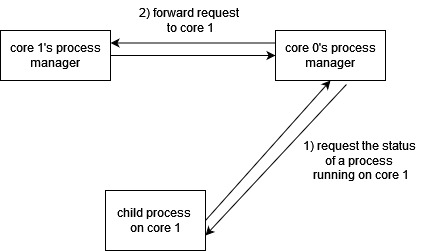
\includegraphics[width=0.8\columnwidth]{images/m6-ump-proc.jpg}
    \caption{The UMP calls that need to be made if the process server could only be contacted via UMP.}
    \label{figure:m6-ump-proc}
\end{figure}
\\\\
Although this seems strange and very roundabout, we hypothesize that despite the overhead of making more RPC calls (via UMP), it would still be faster to do this than to contact the process server through LMP. Our justification for this decision lies in the next section where we look at performance measurements. 

\subsection{Performance Measurements}
Our first question (and probably yours too) was ``is our UMP implementation actually faster than LMP"? To test this, we had a child process send a string of increasing length (which will require increasing numbers of messages, due to our long-message implementation) to \texttt{init} on its local core via LMP. We then compared the latency of these RPC calls with sending the strings to the other core's \texttt{init} via UMP. The results are observed in Figure \ref{figure:send-string-no-kernel}.
\begin{figure}[ht]
    \centering
    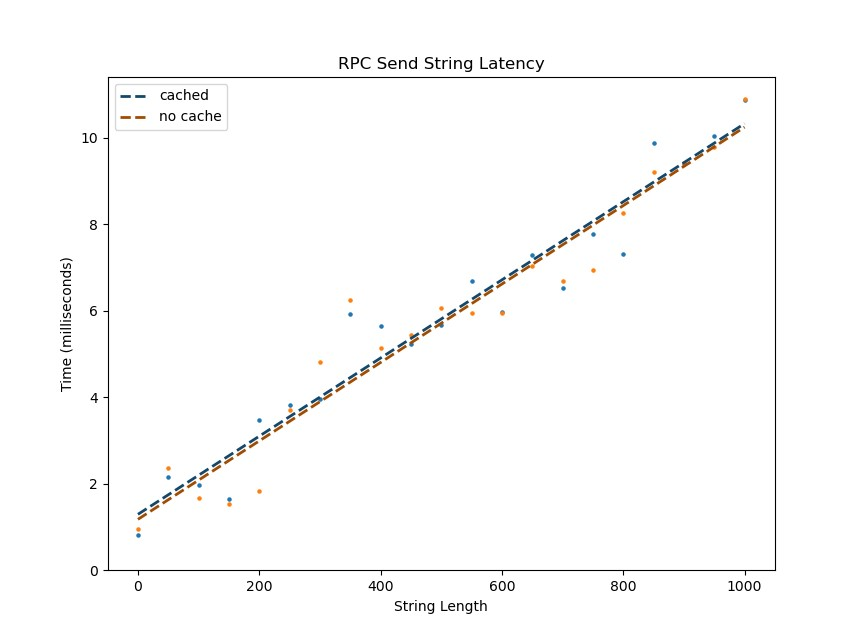
\includegraphics[width=0.8\columnwidth]{images/send-string-no-kernel.png}
    \caption{Sending a string via UMP vs LMP while under no kernel load.}
    \label{figure:send-string-no-kernel}
\end{figure}
\\\\
These are very alarming results. Our UMP implementation does not seem to be much faster than LMP. In fact, LMP also seems quite fast, as both  protocols service the request within approximately 10 milliseconds. We discussed various reasons for observing these results such as whether or not we had implemented UMP properly to exploit the ``MOESI" protocol (which allows us to bypass memory write-backs). 
\\\\
Discussions centered around our code did not lead to anything conclusive until we realized a key piece of information: this test ran on our system in isolation. The kernel was free to deliver and receive LMP messages, as nothing else was causing contention in access to the kernel. Furthermore, UMP also has the overhead of constantly needing to poll its channel for new messages, which would not make it faster in these conditions. We re-ran our tests, now with a simultaneously running thread that constantly used a capability operation requiring kernel involvement. The results are shown in Figure \ref{figure:send-string-kernel}.
\begin{figure}[ht]
    \centering
    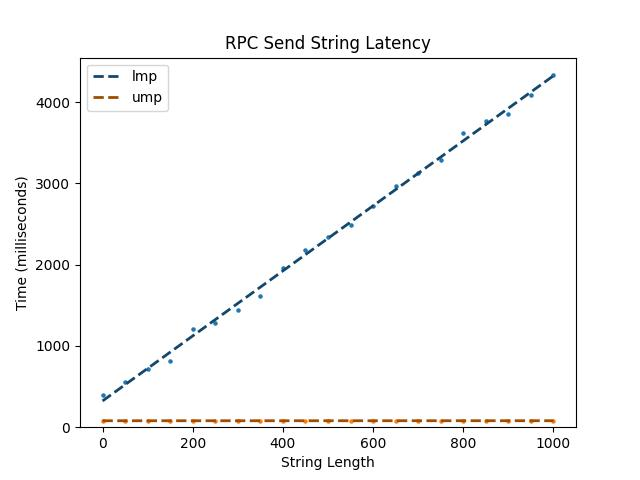
\includegraphics[width=0.8\columnwidth]{images/send-string-kernel.jpg}
    \caption{Sending a string via UMP vs LMP while under high kernel load.}
    \label{figure:send-string-kernel}
\end{figure}
\\\\
These results are much more in line with our expectations of UMP. Using these results, we now tested our hypothesis from the previous section about how processes should communicate with the process management server. Figure \ref{figure:proc-kernel} shows the latency of a process on core \textbf{1} requesting the status of a process running on its local core via LMP compared with UMP. This test was also run with a simulated kernel load.
\begin{figure}[ht]
    \centering
    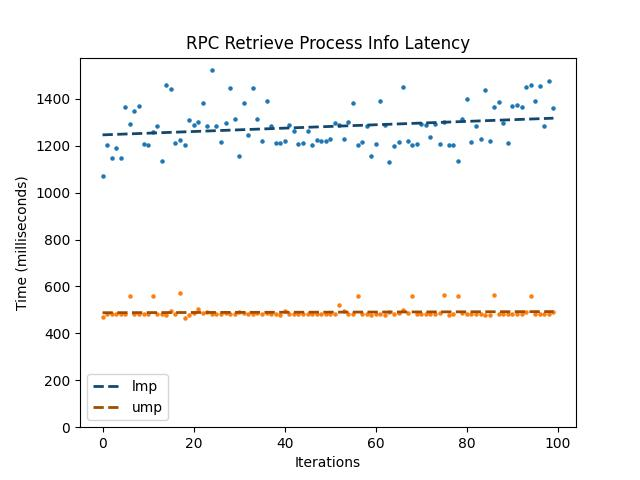
\includegraphics[width=0.8\columnwidth]{images/proc-kernel.jpg}
    \caption{Requesting the status of a process running on the same core via LMP vs UMP, under kernel load.}
    \label{figure:proc-kernel}
\end{figure}
\\\\
UMP is still much faster than LMP under kernel load despite requiring more message passing. We then made our decision to use UMP for contacting process servers based on these observations.
\clearpage
